%%%%%%%%%%%%%%%%%%%%%%%%%%%%%%%%%%%%%%%%%
% Daily Laboratory Book
% LaTeX Template
%
% This template has been downloaded from:
% http://www.latextemplates.com
%
% Original author:
% Frank Kuster (http://www.ctan.org/tex-archive/macros/latex/contrib/labbook/)
%
% Important note:
% This template requires the labbook.cls file to be in the same directory as the
% .tex file. The labbook.cls file provides the necessary structure to create the
% lab book.
%
% The \lipsum[#] commands throughout this template generate dummy text
% to fill the template out. These commands should all be removed when 
% writing lab book content.
%
% HOW TO USE THIS TEMPLATE 
% Each day in the lab consists of three main things:
%
% 1. LABDAY: The first thing to put is the \labday{} command with a date in 
% curly brackets, this will make a new page and put the date in big letters 
% at the top.
%
% 2. EXPERIMENT: Next you need to specify what experiment(s) you are 
% working on with an \experiment{} command with the experiment shorthand 
% in the curly brackets. The experiment shorthand is defined in the 
% 'DEFINITION OF EXPERIMENTS' section below, this means you can 
% say \experiment{pcr} and the actual text written to the PDF will be what 
% you set the 'pcr' experiment to be. If the experiment is a one off, you can 
% just write it in the bracket without creating a shorthand. Note: if you don't 
% want to have an experiment, just leave this out and it won't be printed.
%
% 3. CONTENT: Following the experiment is the content, i.e. what progress 
% you made on the experiment that day.
%
%%%%%%%%%%%%%%%%%%%%%%%%%%%%%%%%%%%%%%%%%

%----------------------------------------------------------------------------------------
%	PACKAGES AND OTHER DOCUMENT CONFIGURATIONS
%----------------------------------------------------------------------------------------

\documentclass[15pt,idxtotoc,hyperref,openany]{labbook} % 'openany' here removes the gap page between days, erase it to restore this gap; 'oneside' can also be added to remove the shift that odd pages have to the right for easier reading

\usepackage{listings}
\usepackage{color}

\definecolor{dkgreen}{rgb}{0,0.6,0}
\definecolor{gray}{rgb}{0.5,0.5,0.5}
\definecolor{mauve}{rgb}{0.58,0,0.82}

\lstset{frame=tb,
  language=C,
  aboveskip=3mm,
  belowskip=3mm,
  showstringspaces=false,
  columns=flexible,
  basicstyle={\small\ttfamily},
  numbers=none,
  numberstyle=\tiny\color{gray},
  keywordstyle=\color{blue},
  commentstyle=\color{dkgreen},
  stringstyle=\color{mauve},
  breaklines=true,
  breakatwhitespace=true
  tabsize=3
}




\usepackage[ 
  backref=page,
  pdfpagelabels=true,
  plainpages=false,
  colorlinks=true,
  bookmarks=true,
  pdfview=FitB]{hyperref} % Required for the hyperlinks within the PDF
  
\usepackage{booktabs} % Required for the top and bottom rules in the table
\usepackage{float} % Required for specifying the exact location of a figure or table
\usepackage{graphicx} % Required for including images
\usepackage{lipsum} % Used for inserting dummy 'Lorem ipsum' text into the template

\newcommand{\HRule}{\rule{\linewidth}{0.5mm}} % Command to make the lines in the title page
\setlength\parindent{0pt} % Removes all indentation from paragraphs

%----------------------------------------------------------------------------------------
%	DEFINITION OF EXPERIMENTS
%----------------------------------------------------------------------------------------

\newexperiment{example}{This is an example experiment}
\newexperiment{example2}{This is another example experiment}
\newexperiment{example3}{This is yet another example experiment}
\newexperiment{table}{This shows a sample table}
%\newexperiment{shorthand}{Description of the experiment}

%---------------------------------------------------------------------------------------

\begin{document}

%----------------------------------------------------------------------------------------
%	TITLE PAGE
%----------------------------------------------------------------------------------------

\frontmatter % Use Roman numerals for page numbers
\title{
\begin{center}
\HRule \\[0.4cm]
{\Huge \bfseries Systems Notes \\[0.5cm] \Large Computer Science}\\[0.4cm] % Degree
\HRule \\[1.5cm]
\end{center}
}
\author{\Huge Alex Norton\\ \\ \LARGE ajn123@vt.edu \\[2cm]} % Your name and email address
\date{Beginning 9 February 2014} % Beginning date
\maketitle

\tableofcontents

\mainmatter % Use Arabic numerals for page numbers

%----------------------------------------------------------------------------------------
%	LAB BOOK CONTENTS
%----------------------------------------------------------------------------------------

% Blank template to use for new days:

%\labday{Day, Date Month Year}

%\experiment{}

%Text

%-----------------------------------------

%\experiment{}

%Text

%----------------------------------------------------------------------------------------

\labday{Chapter 8: Shell}

\experiment{Process}
The first thing to understand is that a {\bf computer program} is a passive collection of instructions; a {\bf process} is the actual execution of those instructions.\\

A {\bf process} in user mode is not allowed to execute privileged instructions.  The only way for the process to change from user mode to kernel mode is via an exception such as an {\bf interrupt}, a {\bf fault} or a {\bf trapping system call}.


Processes can have three states:
\begin{enumerate}
\item  {\bf Running}  The process is currently running on a CPU.
\item {\bf Ready} Process could make progress if CPU were available
\item  {\bf Blocked} Process is waiting for something (memory, signal, time, etc)
\end{enumerate}


%-----------------------------------------

\experiment{Context switching} % Multiple experiments can be included in a single day, this allows you to segment what was done each day into separate categories

In computing, a {\bf context switch} is the process of storing and restoring the state (context) of a process so that execution can be resumed from the same point at a later time. This enables multiple processes to share a single CPU and is an essential feature of a multitasking operating system. What constitutes the context is determined by the processor and the operating system.\\

A context switch follows these 3 steps:

\begin{enumerate}
\item   saves the contents of the current process.
\item  restores the saved context of some previously preempted process
\item  passes control to this newly restored process
\end{enumerate}


\experiment{File Descriptor}

A file descriptor is an indicator for a way of accessing a file.


\experiment{Signal}
A {\bf signal} is a message that notifies a process that an event of some type has occured in the system (just like when you press a button on your phone, a message is sent to the operating system).  Each signal corresponds to some kind of system event.  For example, a signal can be used to cancel background jobs.\\


A pending signal is a signal that has been sent but not recieved.  A process can also block a CERTAIN signal.  In this case, blocked sigals can be sent
but will not be received until the signal is unblocked.


\begin{figure}[H] % Example of including images
\begin{center}
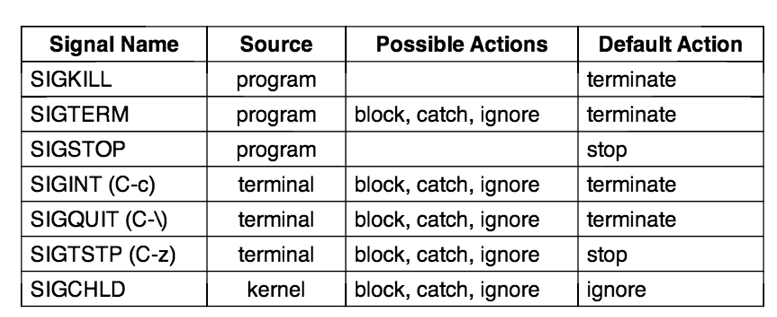
\includegraphics[width=0.5\linewidth]{signals}
\end{center}
\caption{Table of possible signals}
\label{fig:example_figure}
\end{figure}

%-----------------------------------------

\experiment{Pipelining}

Pipelining works by setting the standard output(1) of the first command to the standard input(0) of the second command in the pipeline.  
here are a couple of system calls that you may be interested to understand what is happening in more detail, in particular, fork(2), 
execve(2), pipe(2), dup2(2), read(2) and write(2).

\begin{itemize}
\item The dup2 function takes two parameters $dup2(old, new)$  The pointer of old will replace the pointer of new when the function is called. (code example below)
\end{itemize}


\begin{table}[H]
\begin{tabular}{l l l}
\toprule
\textbf{Integer Value} & \textbf{Name}  \\
\toprule
0 & Standard Input (Stdin)\\
1 & Standard Output (Stdout) \\
2 & Standard Error (Stderr) \\
\bottomrule
\end{tabular}
\caption{Integer Values and their File descriptors}
\label{tab:treatments_xy}
\end{table}


 \newpage
\begin{lstlisting}
1	#include <stdio.h>
2	#include <unistd.h>
3	#include <sys/types.h>
4	
5	#define IN 0
6	#define OUT 1
7	
8	int main(void)
9	{
10	  char string[] = "Hello, world!\n";
11	  char readbuffer[80];
12	
13	  // Creates the pipe using the integer array of size two.
14	  int fd[2];
15	  pipe(fd);
16	
17	  // Fork new process
18	  if(fork() == 0)
19	  {
20	    // Copy the write end of pipe to standard out.
21	    dup2( fd[OUT], OUT );
22	    // Close read and write end of pipe.
23	    close( fd[IN] );
24	    close( fd[OUT] );
25	    // Child Process: execute new process
26	    char *cmd[] = {"ls", "-la", (char *) 0};
27	    execvp("ls", cmd);
28	  }
29	  else
30	  {
31	    // Clise write end of pipe.
32	    close( fd[OUT] );
33	    // Parent Process: Read string from the read side of pipe.
34	    read( fd[IN], readbuffer, sizeof(readbuffer) );
35	    printf("Received string: %s", readbuffer);
36	  }
37	  return(0);
38	}
\end{lstlisting}

 \newpage
\experiment{Fork}

This is an example of the fork method in C.  fork() clones a process from a process.  This new process can be used to execute another process or
do other things.  NOTE:  Once you clone a process you have no idea which order your clones will run in, your code should not depend on the order.  Another thing to remember is that fork returns twice, once in the parent and once in the child (the new process you just created).  The cloned process is exactly the same except for the return value of fork().  In the child process fork will always return 0 and in the parent it will return the process ID of itself so your code can just check for the child process with == 0 and the parent with an else.\\

Fork returns the PROCESS ID OF ITS CHILD to the parent process, so that the parent knows its PID of the child to keep track of it.  Fork() returns 0 to the child, you don't need it.
\begin{lstlisting}
#include <unistd.h>
#include <stdio.h>

int main(){
	int x = 1;
	
	int pid = fork();// pid contains the childs pid for the parent process.
	if (pid== 0) 
	{// only child executes this
		printf("Child, x = %d\n", ++x);
	} 
	else {
	// only parent executes this
		printf("Parent, x = %d\n", --x);
	}// parent and child execute this
	printf("Exiting with x = %d\n", x);
	return 0;
}
\end{lstlisting}

\experiment{reentrant}


A computer program in {\bf reentrant} if it can be interrupted in the middle of its execution and then safely called again.  An interuption can come from a signal or a jump.  Once the reentered invocation completes, the previous invocations will resume correct execution.

\begin{itemize}
\item Printf() is a NON reentrant function, meaning that it is not safe to interrupt.
\end{itemize}

\experiment{Signal Handlers}
Signal handlers are used to deal with the different types of signals on a USER LEVEL.\\

When a handler function is invoked on a signal, that signal is automatically blocked (in addition to any other signals that are already in the process's signal mask) during the time the handler is running. \\




\experiment{PID-process identifier}
A number used to temporarily uniquely identify a process.\\
One may use the command "ps j" to see PPID (parent process ID), PID (process ID), PGID (process group ID) and SID (session ID) of processes.   \\

Every process can have a PID, parent ID, and a group ID(gid).  A group ID means that all of the processes share the terminal together and you do not need to transfer control for these processes.  When you send a signal to a terminal, everything in the terminal control group (same gid) will receive that signal. When you send a signal via kill(), it depends on how you structure the arguments.

%----------------------------------------------------------------------------------------

\labday{Thread Pool}

\experiment{Threads}
A {\bf Thread} is a logical flow that runs in the context of the program.  Threads share all the same date structures (virtual address space), processes DO NOT.  It is also important to note that each thread has its own thread context including a unique integer thread ID (TID), stack,stack pointer, program counter, general purpose registers, and condition codes.\\

threads  are scheduled automatically by the kernel and are known by an integer ID.\\
Each process begins life as a single thread called the main thread.  At some point the main thread creates a peer thread, and from this point in time the two threads run concurrently.  Eventually ,control passes to the peer thread via a context switch , because the main thread is doing something slow (read, sleep, or disk access)\\

Threads are organized in a pool of peers.  The main thread is different in that it is always the first thread to run in the process.  Each peer can read and write the same shared data.\\

Variables in threaded C programs are mapped to virtual memory according to their storage classes:
\begin{itemize}
\item Global Variables (Shared):  A global variable is any variable declared outside of a function.  At run, the read/write area of virtual memory contains exactly one instance of each global variable that can be referenced by any thread.
\item Local Automatic Variables (Not Shared): This is a variable declared inside a function WITHOUT the static attribute.  At run time, each thread's stack contains its own instances of any local automatic variables.
\item Local Static Variables (Shared):  This is a variable declared inside a function with the static attribute.  As with global variables , the read/write area of virtual memory contains exactly one instance of each local static variable in our program.
\end{itemize}


\begin{lstlisting}
#include <stdio.h>
#include <pthread.h>

#define NUMTHRDS 2

pthread_t t [ NUMTHRDS];
int coin_flip;

pthread_mutex_t flip_done;
static void *thread2(void *_){
	pthread_mutex_lock(&flip_done);
	printf("Thread 2: flipped coin %d\n", coin_flip);
}


static void * thread1(void * _)
{
	coin_flip = 1;
	pthread_mutex_unlock(&flip_done);
	printf("Thread 1: flipped coin %d\n", coin_flip);
}
int main()
{
	pthread_mutex_init(&flip_done, NULL);
	pthread_mutex_lock(&flip_done);
	pthread_create(&t[1], NULL, thread2, NULL);
	pthread_create(&t[0], NULL, thread1, NULL);
	 pthread_mutex_destroy(&flip_done);
	//must have this as main will block until all the supported threads are done
	pthread_exit(NULL);
	return 1;
}


\end{lstlisting}


\experiment{Race Conditions}
One thing to watch out for in threads is a race condition.  A race condition occurs when two or more threads read and write a shared variable, and the final result depends on the execution of those threads.

\experiment{Semaphores}
A semaphore is a variable or abstract data type that is used for controlling access to multiple threads or processes

Semaphores provide a great way to ensure mutuaally exclusive access to shared variables.  A semaphore that is used to protect shared variables is called a binary semaphore becuase its value is always 0 or 1.\\

Another important use of semaphores ,besides providing mutual exclusion, is to schedule accesses to shared rescources.\\

Think of semaphores as bouncers at a nightclub. There are a dedicated number of people that are allowed in the club at once. If the club is full no one is allowed to enter, but as soon as one person leaves another person might enter.



\labday{Memory Allocation}

\experiment{Start}



\labday{Web Server}

Here are some definitions to start:
\begin{itemize}
\item {\bf URI (Uniform Recsource Identifier}- The suffix of the corresponding URS that includes the filename and optional arguments.
\item {\bf Network Port}- A number signaling what different type of traffic is sent over (email, internet, texts).  Ports talk to other devices as well as other networks through these ports.  
\item {\bf Sockets}- Let the client and server talk over ports by providing an API that allows communication between the server and the client.  Sockets talk to applications.
\end{itemize}

\experiment{Protocol Layering}
A {\bf  protocol } is a set of layers used to communicate with eachother.  Each instance of a protocol talks virtually to its peer using the protocol.  Each instance of a protocol uses only the servicese of a lower layer.  Protocols must provide two things:
\begin{itemize}
\item Provides a naming scheme for host addresses, a unique address to identify itself.
\item Provide a delivery mechanism called a packet which consists of a header and a payload.  Header contains size, source, and destination.  Payload contains bits sent from source.
\end{itemize}


\begin{figure}[H] % Example of including images
\begin{center}
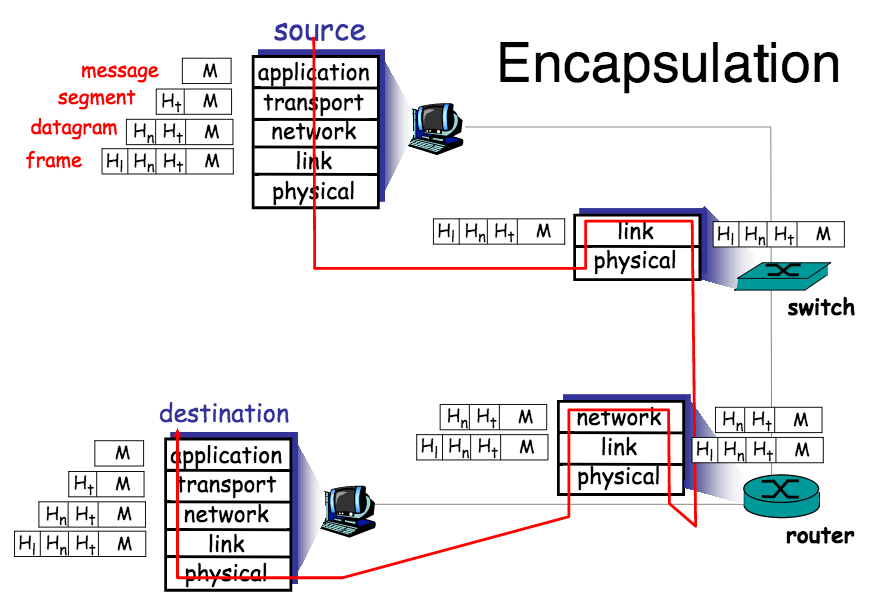
\includegraphics[width=.8\linewidth]{encapsulation}
\end{center}
\caption{How protocol layering works}
\label{fig:example_figure}
\end{figure}


\begin{table}[H]
\begin{tabular}{l l l}
\toprule
\textbf{Groups} & \textbf{Treatment X} & \textbf{Treatment Y} \\
\toprule
1 & 0.2 & 0.8\\
2 & 0.17 & 0.7\\
3 & 0.24 & 0.75\\
4 & 0.68 & 0.3\\
\bottomrule
\end{tabular}
\caption{The effects of treatments X and Y on the four groups studied.}
\label{tab:treatments_xy}
\end{table}

Table \ref{tab:treatments_xy} shows that groups 1-3 reacted similarly to the two treatments but group 4 showed a reversed reaction.

%----------------------------------------------------------------------------------------

\labday{Saturday, 27 March 2010}

\experiment{Bulleted list example} % You don't need to make a \newexperiment if you only plan on referencing it once

This is a bulleted list:

\begin{itemize}
\item Item 1
\item Item 2
\item \ldots and so on
\end{itemize}

%-----------------------------------------

\experiment{example}

\lipsum[6]

%-----------------------------------------

\experiment{example2}

\lipsum[7]

%----------------------------------------------------------------------------------------
%	FORMULAE AND MEDIA RECIPES
%----------------------------------------------------------------------------------------

\labday{} % We don't want a date here so we make the labday blank

\begin{center}
\HRule \\[0.4cm]
{\huge \textbf{Formulae and Media Recipes}}\\[0.4cm] % Heading
\HRule \\[1.5cm]
\end{center}

%----------------------------------------------------------------------------------------
%	MEDIA RECIPES
%----------------------------------------------------------------------------------------

\newpage

\huge \textbf{Media} \\ \\

\normalsize \textbf{Media 1}\\
\begin{table}[H]
\begin{tabular}{l l l}
\toprule
\textbf{Compound} & \textbf{1L} & \textbf{0.5L}\\
\toprule
Compound 1 & 10g & 5g\\
Compound 2 & 20g & 10g\\
\bottomrule
\end{tabular}
\caption{Ingredients in Media 1.}
\label{tab:med1}
\end{table}

%-----------------------------------------

%\textbf{Media 2}\\ \\

%Description

%----------------------------------------------------------------------------------------
%	FORMULAE
%----------------------------------------------------------------------------------------

\newpage

\huge \textbf{Formulae} \\ \\

\normalsize \textbf{Formula 1 - Pythagorean theorem}\\ \\
$a^2 + b^2 = c^2$\\ \\

%-----------------------------------------

%\textbf{Formula X - Description}\\ \\

%Formula

%----------------------------------------------------------------------------------------

\end{document}